\begin{description}
	\item[Description] Small synthetic data set from Lauritzen S. and Spiegelhalter D. (1988) about lung diseases (tuberculosis, lung cancer or bronchitis) and visits to Asia.

	\item[Number of nodes] 8
	
	\item[Number of arcs] 8
	
	\item[Number of parameters] 18
\end{description}

Lauritzen S. and Spiegelhalter D. (1988) motivate this example as follows:

"Shortness-of-breath (dyspnoea) may be due to tuberculosis, lung cancer or bronchitis, or none of them, or more than one of them. A recent visit to Asia increases the chances of tuberculosis, while smoking is known to be a risk factor for both lung cancer and bronchitis. The results of a single chest X-ray do not discriminate between lung cancer and tuberculosis, as neither does the presence or absence of dyspnoea."

\begin{table}[p]
\centering	\caption{Comparison of scores and correct arcs via Asia data set} \tiny	
{\tabcolsep=0.01in
	\begin{tabular}{cc||cc|cc|cc||cc|cc|cc|cc}
		\hline	
		& & \multicolumn{14}{c}{Asia (Num of Nodes = 8)}\tabularnewline	
		\hline	
		\multicolumn{2}{c||}{Sample Size} & \multicolumn{2}{c|}{1000} & \multicolumn{2}{c|}{5000} & \multicolumn{2}{c||}{10000} & & & \multicolumn{2}{c|}{1000} & \multicolumn{2}{c|}{5000} & \multicolumn{2}{c}{10000}\tabularnewline	
		\hline	
		& & Sum. & Std.Dev. & Sum. & Std.Dev. & Sum. & Std.Dev. & & & Sum. & Std.Dev. & Sum. & Std.Dev. & Sum. & Std.Dev.\tabularnewline
		\hline	
		\hline	
		\multirow{4}{*}{BDe} & HC & -229814 & 35.25 & -1113883 & 85.65 & -2218508 & 126.41 & \multirow{4}{*}{C} & HC & 677 & 0.55 & 716 & 0.37 & 735 & 0.48\tabularnewline	
		& TABU & -229806 & 35.29 & -1113857 & 85.9 & -2218431 & 126.4 & & TABU & 655 & 0.73 & 677 & 0.72 & 703 & 0.76\tabularnewline	
		& MMHC & -249829 & 41.68 & -1213021 & 117.02 & -2417769 & 191.84 & & MMHC & 461 & 0.55 & 503 & 0.48 & 514 & 0.59\tabularnewline	
		& RSMAX2 & -252800 & 43.81 & -1233095 & 121.09 & -2457976 & 173.35 & & RSMAX2 & 400 & 0 & 400 & 0 & 400 & 0\tabularnewline	
		\hline	
		\multirow{4}{*}{loglik} & HC & -220520 & 36.46 & -1102564 & 85.92 & -2206160 & 126.05 & \multirow{4}{*}{M} & HC & 122 & 0.52 & 83 & 0.38 & 65 & 0.48\tabularnewline	
		& TABU & -220505 & 36.54 & -1102521 & 86.31 & -2206030 & 126.02 & & TABU & 122 & 0.52 & 83 & 0.38 & 65 & 0.48\tabularnewline	
		& MMHC & -241431 & 43.03 & -1202710 & 117.97 & -2406616 & 192.19 & & MMHC & 339 & 0.55 & 297 & 0.48 & 286 & 0.59\tabularnewline	
		& RSMAX2 & -244901 & 44.97 & -1223631 & 121.63 & -2447783 & 173.8 & & RSMAX2 & 400 & 0 & 400 & 0 & 400 & 0\tabularnewline	
		\hline	
		\multirow{4}{*}{AIC} & HC & -222238 & 36.46 & -1104349 & 85.87 & -2208092 & 126.21 & \multirow{4}{*}{WO} & HC & 1 & 0.1 & 1 & 0.1 & 0 & 0\tabularnewline	
		& TABU & -222226 & 36.53 & -1104315 & 86.16 & -2207985 & 126.19 & & TABU & 23 & 0.51 & 40 & 0.62 & 32 & 0.66\tabularnewline	
		& MMHC & -242973 & 43 & -1204336 & 117.81 & -2408295 & 192.1 & & MMHC & 0 & 0 & 0 & 0 & 0 & 0\tabularnewline	
		& RSMAX2 & -246201 & 44.97 & -1224936 & 121.62 & -2449114 & 173.8 & & RSMAX2 & 0 & 0 & 0 & 0 & 0 & 0\tabularnewline	
		\hline	
		\multirow{4}{*}{BIC} & HC & -226454 & 36.49 & -1110166 & 85.76 & -2215057 & 126.96 & \multirow{4}{*}{WC} & HC & 72 & 1.22 & 96 & 1.12 & 224 & 1.69\tabularnewline	
		& TABU & -226449 & 36.52 & -1110161 & 85.76 & -2215033 & 126.99 & & TABU & 112 & 1.43 & 170 & 1.46 & 292 & 2.02\tabularnewline	
		& MMHC & -246757 & 42.97 & -1209634 & 117.34 & -2414348 & 191.83 & & MMHC & 202 & 0.2 & 218 & 0.58 & 244 & 0.83\tabularnewline	
		& RSMAX2 & -249391 & 44.97 & -1229189 & 121.6 & -2453913 & 173.82 & & RSMAX2 & 0 & 0 & 8 & 0.39 & 50 & 0.87\tabularnewline	
		\hline	
	\end{tabular}
}
\end{table} 

	\begin{figure}[p]
	\centering
		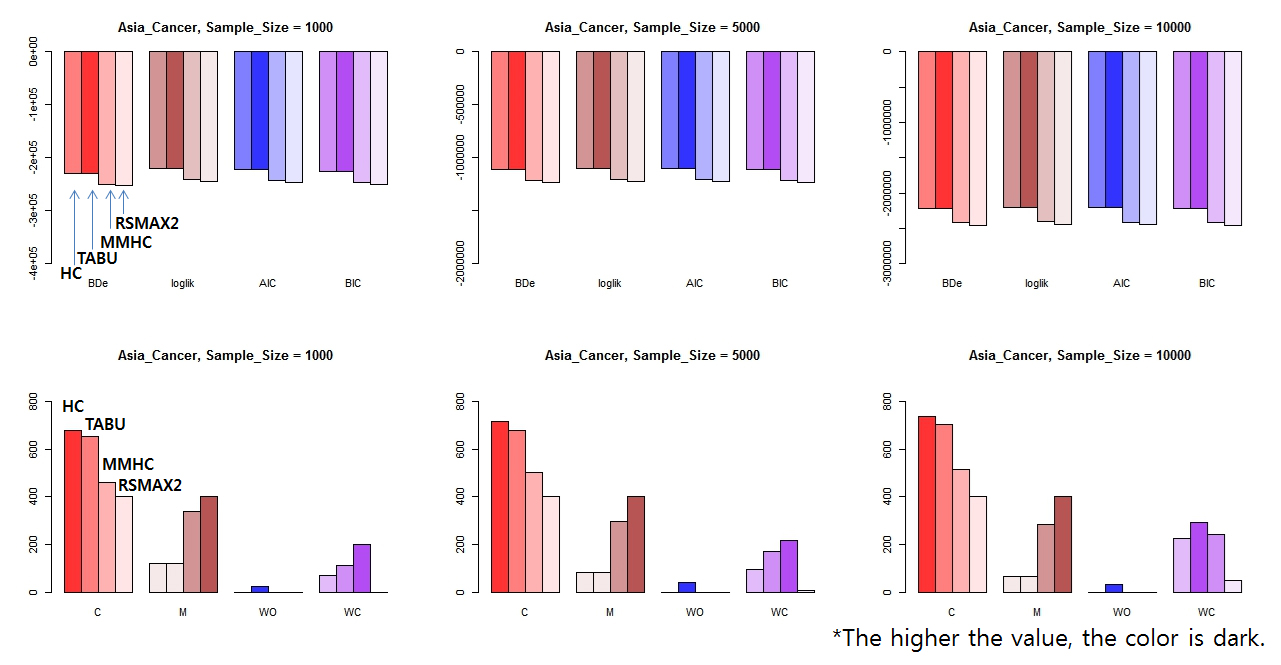
\includegraphics[height=220pt]{images/Real_1_Asia}
		\caption{Comparison of scores and correct arcs via Asia data set}
	\end{figure}	